\documentclass[]{IEEEtran}
% some very useful LaTeX packages include:
%\usepackage{cite}      
\usepackage{graphicx}   
\usepackage{subfigure} 
\usepackage{url}       
\usepackage{amsmath}    
\usepackage{caption2}
% Your document starts here!
\begin{document}

% Define document title and author
	\title{Weekly Report}
	\author{Adviser: Prof. Yang Wen \\Student: Cheng Wensheng\\ Period: 2018.5.4-5.11
	}
	\markboth{Visual Information Processing Group}{}
	\maketitle

% Write abstract here
\begin{abstract}
	This week I mainly put my effort on improving CETC 54 software and reviewing the Geoscience and Remore Sensing Letters paper.
\end{abstract}

% Each section begins with a \section{title} command
\section{Paper Review}
	% \PARstart{}{} creates a tall first letter for this first paragraph
	\PARstart{T}{he} author proposed a method to combine patch-CNN with deep autoencoder(DAE) on polarimetric SAR classification. The author did experiments to show that patch-CNN method can get better classification accuracy while deep autoencoder can acquire more accurate region texture. The proposed method gets improved classification accuracy and region texture than both.
	
	The major concerns are the novelty and the contribution to remote sensing field. As far as I know, the classification of remote sensing images using patch-CNN or DAE is a very common practice. There are a number of works using even more fashion CNN frameworks, like ResNet, Inception, etc., and improved autoencoder methods, such as sparse autoencoder, denoising autoencoder. While the author barely uses the very basic networks of CNN and autoencoder. The innovation point is the way the author combines patch-CNN and DAE. The integrating method is comparing output probabilities of patch-CNN and DAE with fixed threshold, then choose one of them. This method is relatively rough and not so heuristic, besides it’s really troublesome cause you need to set different thresholds by hand for every classified category. 
	
	The second problem is about the experiment. Since the author has the fully polarimetric SAR data, I couldn’t find the reason why the author just uses HH polarization SAR image for patch-CNN. I recommend to use the pseudo color image taking use of all polarization information. Moreover, in fact this is a semantic segmentation problem, so the author should add the experiment which uses fashion CNN-based semantic segmentation frameworks, like SegNet, DeepLab V3 on the pseudo color image. Then it would be more convincing. 
	
	Fig.~\ref{fig:mp} is the DAE flowchart. Fig.~\ref{fig:ss} is the experiment results.

\newpage
\begin{figure}[!hbt]
%		 Center the figure.
		\vspace{0.2cm}
%		\hspace{50cm}
		\begin{center}
			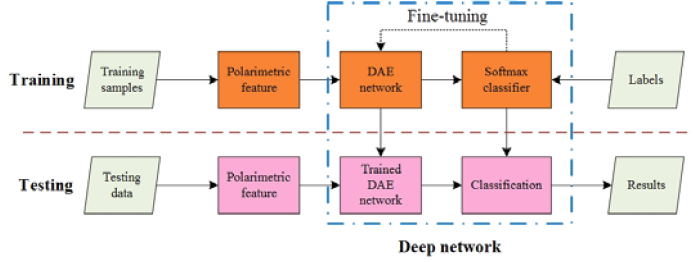
\includegraphics[width=\columnwidth]{DAE}
				%		 Create a subtitle for the figure.
			\caption{The DAE flowchart}
			\label{fig:mp}
		    \vspace{0.2cm}
			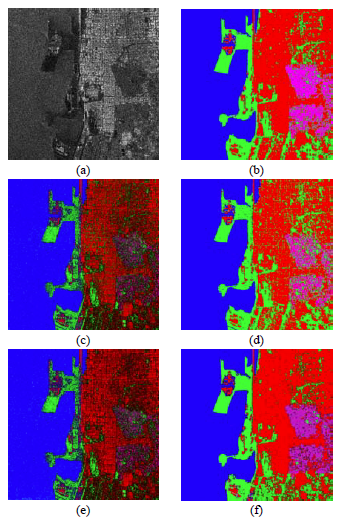
\includegraphics[width=\columnwidth]{out}
				%Create a subtitle for the figure.
			\caption{Experiment results.(a) Original SAR image. (b)
				CNN method. (c) DAE method. (d) Proposed method. (e) SVM method. (f)	MLP method.}
			\label{fig:ss}
		\end{center}
	\end{figure}

% Your document ends here!
\end{document}